\documentclass{beamer}
\usetheme{Oxygen}
\usepackage{graphicx}
\title{\small Desarrollo de un prototipo de robot humanoide que busque, encuentre y patee
una pelota de forma aut\'onoma e inteligente}
\author{Jennifer Dos Reis y Juliana Le\'{o}n \linebreak Tutor Acad\'emico \linebreak Ivette Carolina Mart\'inez }
\begin{document}
\fontfamily{tahoma}
\frame{\titlepage}

\section*{}
\begin{frame}
  \frametitle{\'{I}ndice}
  \tableofcontents[section=1,hidesubsections]
\end{frame}

\AtBeginSection[]
{
  \frame<handout:0>
  {
    \frametitle{\'{I}ndice}
    \tableofcontents[currentsection,hideallsubsections]
	  }
}

\AtBeginSubsection[]
{
  \frame<handout:0>
  {
    \frametitle{\'{I}ndice}
    \tableofcontents[sectionstyle=show/hide,subsectionstyle=show/shaded/hide]
  }
}

\newcommand<>{\highlighton}[1]{%
  \alt#2{\structure{#1}}{{#1}}
}

\newcommand{\icon}[1]{\pgfimage[height=1em]{#1}}

\section{Introducci\'{o}n}

\begin{frame}
  \frametitle{Introducci\'{o}n}
  \begin{block}{}
  \begin{itemize}
    \item Futuro de la robótica 
    \item Algunos ejemplos
    \item Competencia Robocup
  \end{itemize}
  \end{block}

\begin{figure}

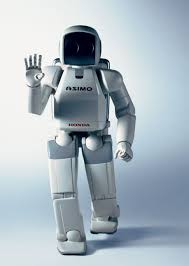
\includegraphics[scale=0.3]{asimo.jpg} 
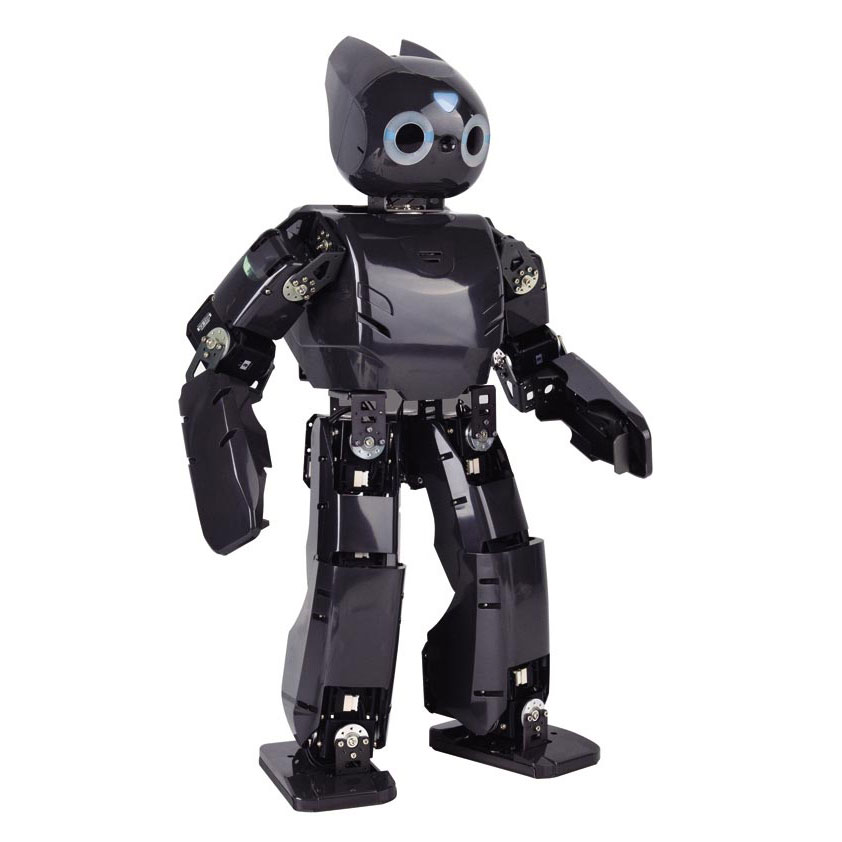
\includegraphics[scale=0.1]{Darwin_OP.jpg} 
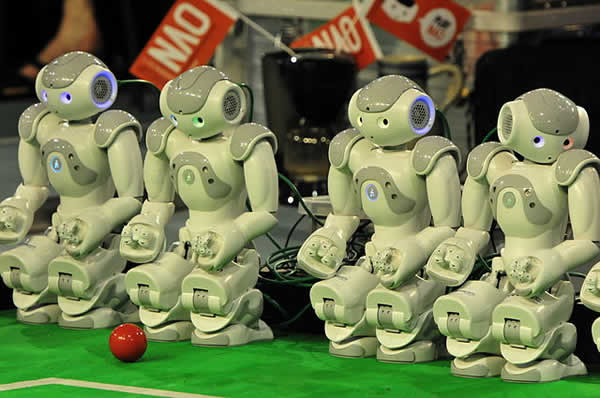
\includegraphics[scale=0.5]{13-06-28-robocup-eindhoven.jpg} 

\end{figure}
\end{frame}

\section{Objetivos}
\begin{frame}
  \frametitle{Objetivos}
  \framesubtitle{Objetivo General}

  \begin{block}{Objetivo General}
	Dise\~nar y construir un robot humanoide capaz de detectar, buscar y patear al arco pelotas de forma aut\'onoma e inteligente
   \end{block}
\end{frame}
\begin{frame}
  \frametitle{Objetivos}
  \framesubtitle{Objetivos Espec\'{i}ficos}
  \begin{block}{Objetivos Espec\'{i}ficos}
  \begin{itemize}
    \item Dise\~no y ensamblaje
    \item Instalaci\'on y configuraci\'on de los componentes 
    \item Detectar la pelota
    \item Desplazamiento 
    \item Control de caidas
    \item Control inteligente de comunicaci\'on
    \item Aprendizaje por reforzamiento 
    \item Orientaci\'on al arco 
    \end{itemize}
  \end{block}
\end{frame}


  

\section{Construci\'on }
\begin{frame}
  \frametitle{Construci\'on}


\begin{block}{Ensamblaje}
	\begin{itemize}
		\item Con piezas de LEGO
		\item Desde cero
		\item Con el kit de piezas Bioloid
	\end{itemize}
\end{block}

 
\end{frame}

\begin{frame}
\begin{block}{Componentes de Junny}
\begin{itemize}
\item Motores Dynamixel
\item Bateria de polimero de Litio
\item Giroscopio 
\item Tarjeta controladora Arbotix
\item Raspberry Pi
\item C\'amara
\item Micro servo motores 
\item chip FTDI
\end{itemize}
\end{block}
\end{frame}

\begin{frame}
\frametitle{Construcci\'on}
\begin{block}{Detecci\'on}
	\begin{itemize}
		\item Anclajes
		
	\end{itemize}
\end{block}

\begin{block}{Desplazamiento}
	\begin{itemize}
	\item Escenas
	\item Personal
	\item Locaci\'{o}n
\end{itemize}		
\end{block}
\end{frame}
\section{Experimentos y Resultados}
\begin{frame}
  \frametitle{Experimentos}
  
  \begin{block}{Simples}
		\begin{itemize}
		\item Herradura
		\item Embobinado con cuerda
		\item Embobinado con cinta tubular
		\item Pasa 3 hala 2
 		\end{itemize}
	   \end{block}
\begin{block}{Compuestos}
	\begin{itemize}
		\item Lote estandar en cuerdas
		\item Equipo de Protecci\'{o}n Personal
	\end{itemize}
\end{block}
\end{frame}

\begin{frame}
\frametitle{Experimentos}
\begin{block}{Completos}
	\begin{itemize}
		\item Ascenso
		
	\end{itemize}
\end{block}
\end{frame}

\section{Conclusiones}
\begin{frame}
\frametitle{Conclusiones}
\begin{block}{Accesibilidad}

\end{block}


\end{frame}
\section{Recomendaciones}
\begin{frame}
\frametitle{Recomendaciones}
\begin{block}{Recomendaciones}

\end{block}
\end{frame}
\begin{frame}

\LARGE{PREGUNTAS}
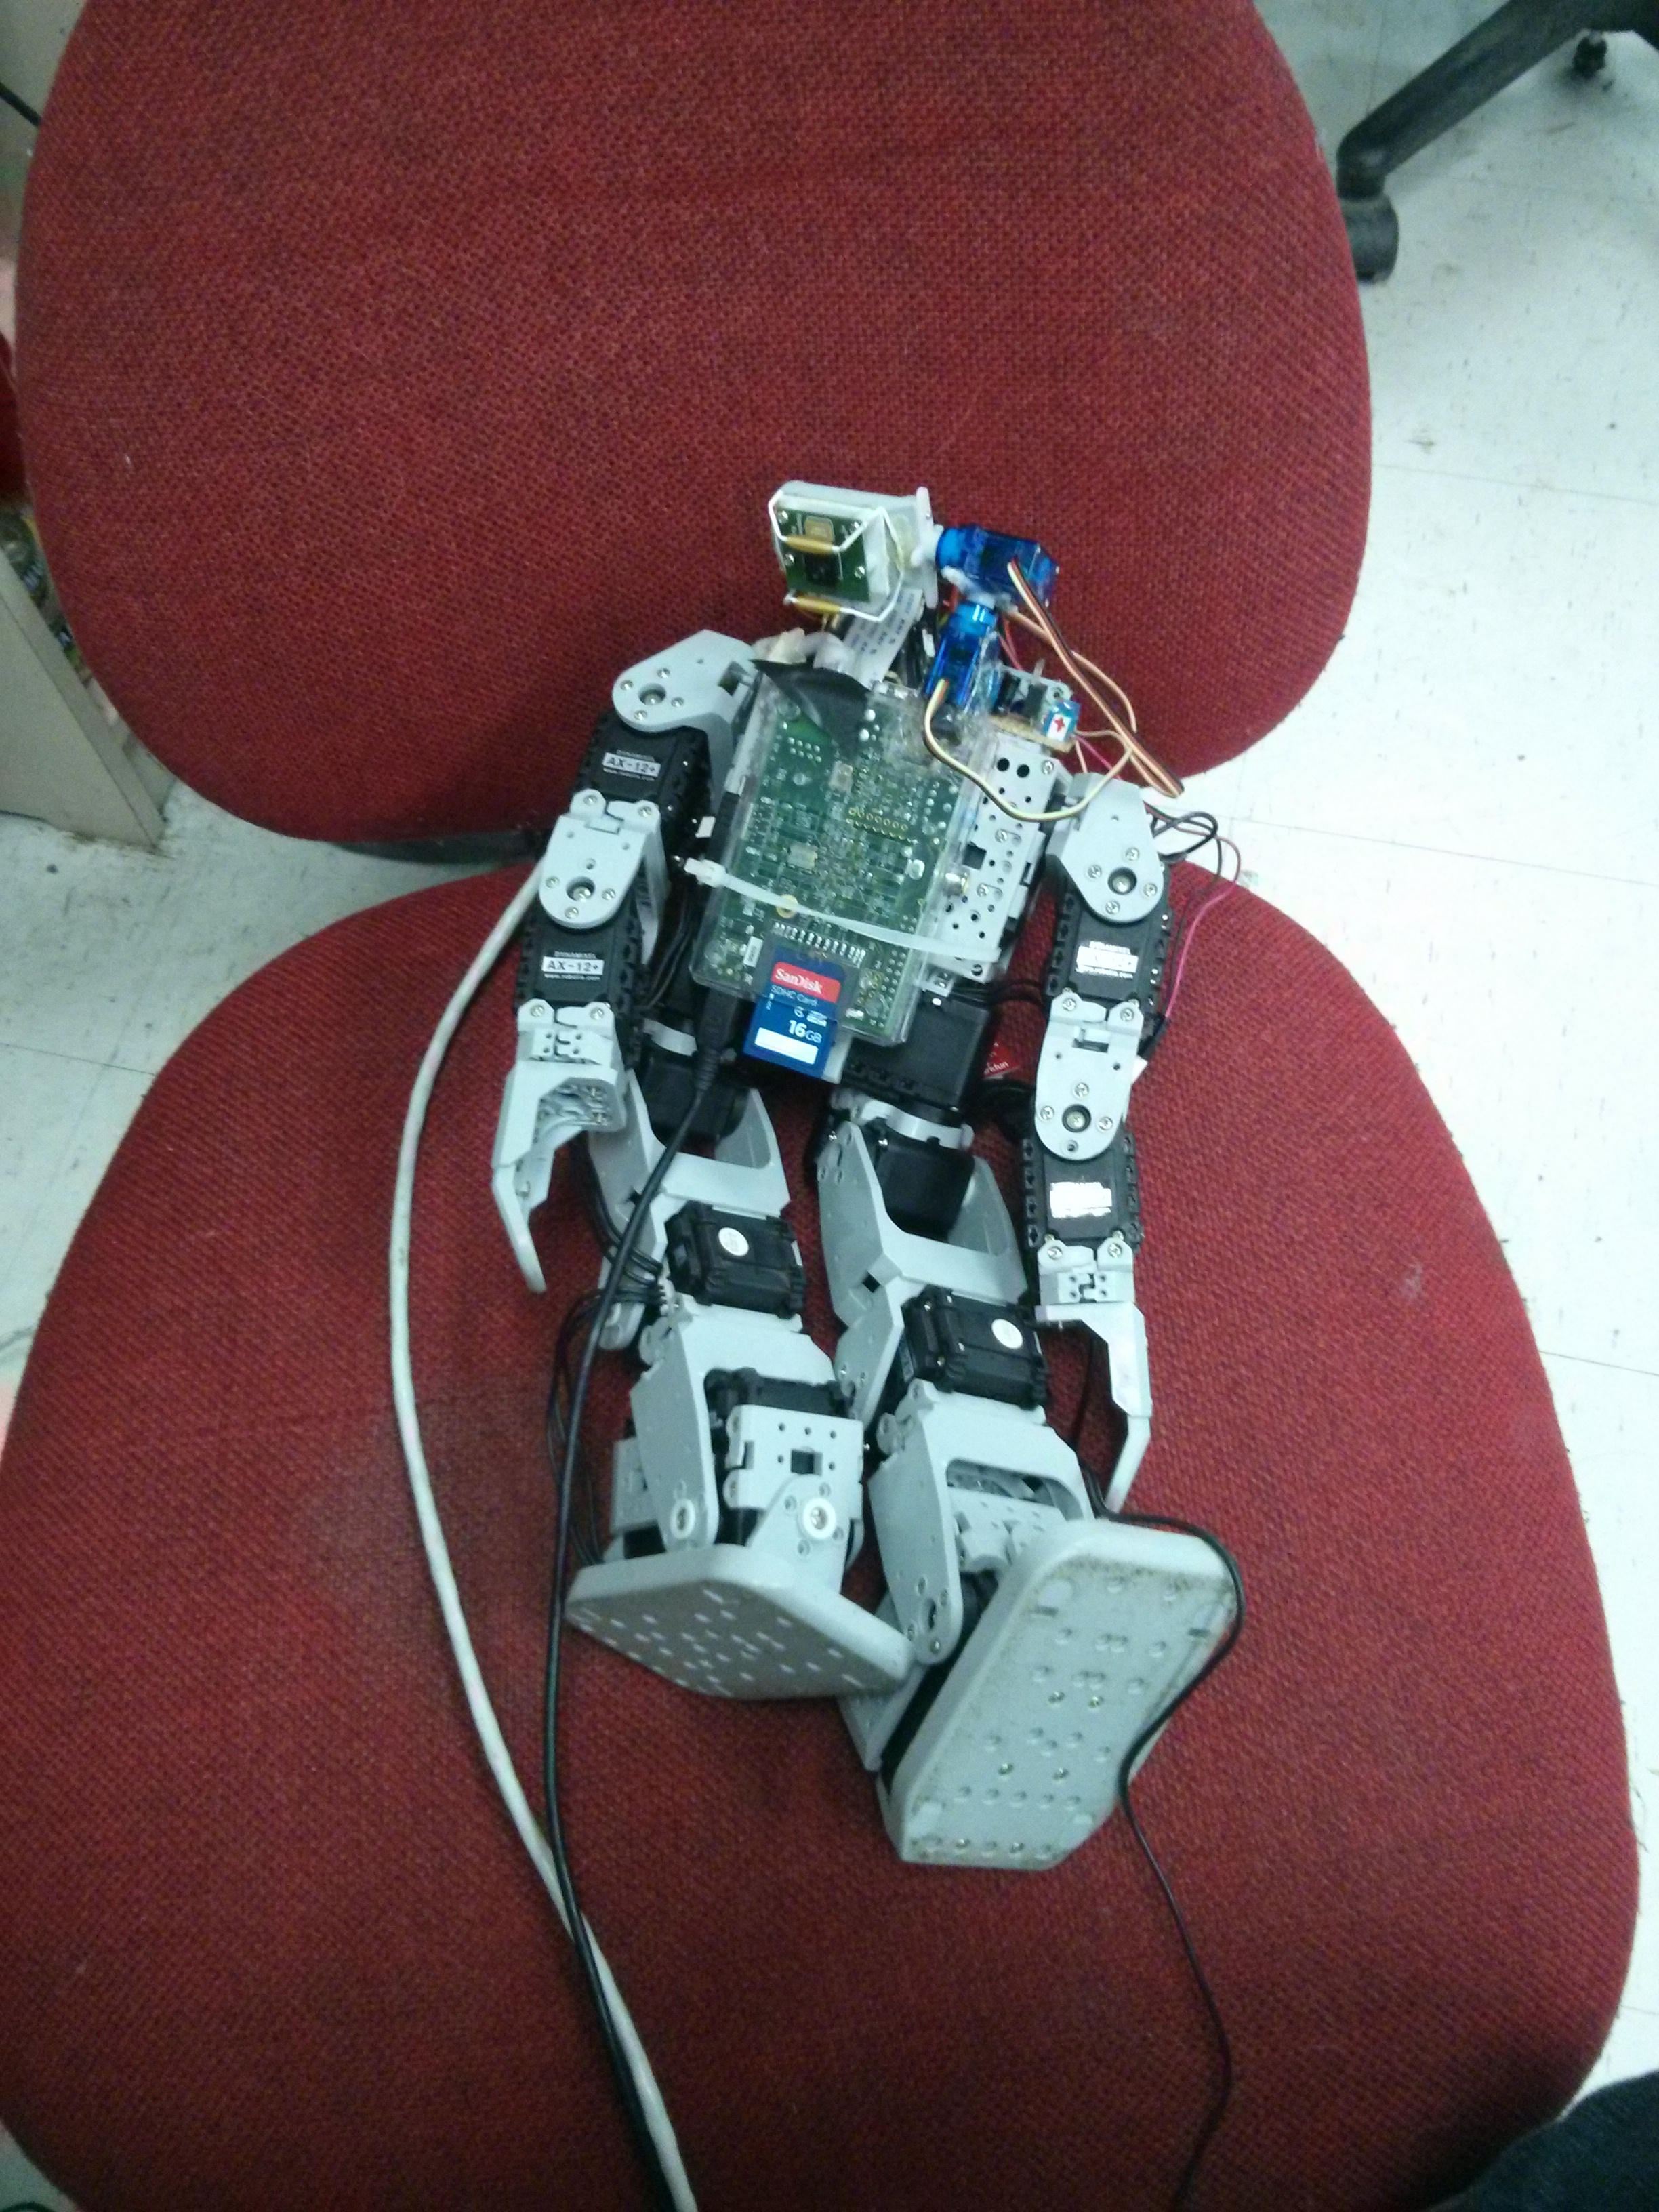
\includegraphics[scale=0.25]{tirolesa}
\end{frame}
\end{document}